\chapter{Περιγραφή Συστήματος}

\section{Εισαγωγή}
Βασικός στόχος αυτού του κεφαλαίου είναι να παρουσιάσει αναλυτικά τις μεθόδους με τις οποίες υλοποιήθηκε το σύστημα. Το σύστημα αποτελείται από 3 κύρια επίπεδα υλοποίησης. Το ανώτερο επίπεδο είναι η διεπαφή των χρηστών ή αλλιώς το γραφικό περιβάλλον το οποίο χωρίζεται σε 2 μέρη. Πρώτο είναι η εφαρμογή κινητών συσκευών και δεύτερο η διαδικτυακή εφαρμογή για τις υπηρεσίες υγείας. Στο αμέσως επόμενο επίπεδο είναι ο εξυπηρετητής ο οποίος περιέχει την υλοποίηση του μοντέλου καθώς και το business logic της εφαρμογής. Τέλος στο κατώτερο επίπεδο βρίσκεται η βάση δεδομένων η οποία είναι υπεύθυνη για την αποθήκευση των δεδομένων ολόκληρου του συστήματος.

\begin{figure}[h]
  \centering
  \includegraphics[width=110mm]{images/system.png}
  \caption{Επισκόπηση συστήματος πτυχιακής}
  \label{fig:system}
\end{figure}

\section{Γραφικό περιβάλλον}
Για το σχεδιασμό του γραφικού περιβάλλοντος των δύο εφαρμογών μας, δόθηκε ιδιαίτερη βάση στην εμφάνιση ώστε να παρέχει μια φιλική αίσθηση στο χρήστη κατά τη διάρκεια λειτουργίας της εφαρμογής. Για το σχεδιασμό του περιβάλλοντος ακολουθήσαμε μια απλοϊκή προσέγγιση με βασική αρχή την παραμονή του γραφικού περιβάλλοντος καθαρού χωρίς μεγάλο αριθμό ενεργειών σε κάθε παράθυρο. Παρακάτω θα γίνει ανάλυση των εργαλείων που χρησιμοποιήθηκαν για να επιτευχθούν οι παραπάνω στόχοι. 

\subsection{Εφαρμογή κινητών συσκευών}
Η εφαρμογή υλοποιήθηκε με τη χρήση του Ionic framework. Το Ionic framework προσφέρει έναν αριθμό εξαρτημάτων για τη διευκόλυνση της δημιουργίας του γραφικού περιβάλλοντος σε κινητές συσκευές. Η χρήση των εξαρτημάτων γίνεται με τη χρήση HTML και CSS. Το Ionic framework ύστερα φροντίζει ώστε το αποτέλεσμα να είναι φιλικό απέναντι στις διαφορετικές πλατφόρμες συσκευών. Στο διάγραμμα ~\ref{fig:ionic-modules} παρουσιάζεται μια σειρά από διαφορετικά παράθυρα μιας εφαρμογής για να γίνει κατανοητό πως εμφανίζεται ένα γραφικό περιβάλλον το οποίο έχει παραχθεί με τη χρήση των Ionic εξαρτημάτων.

\begin{figure}[h]
  \centering
  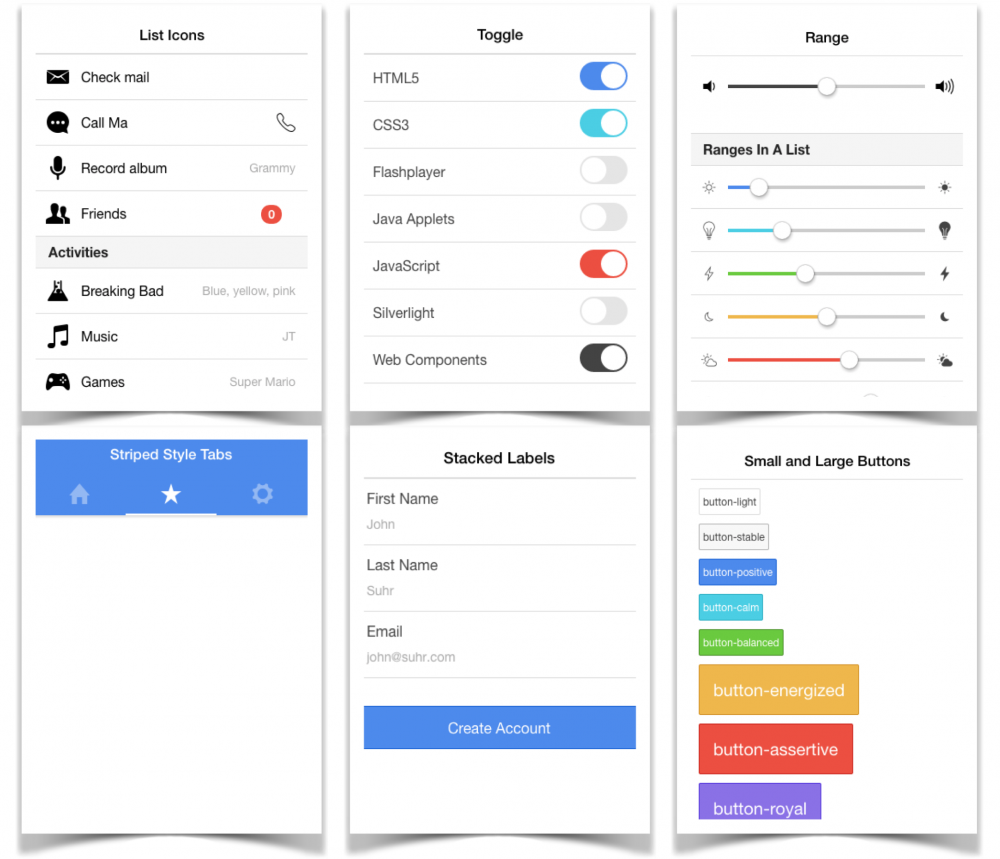
\includegraphics[width=100mm]{images/ionic.png}
  \caption{Επισκόπηση Ιonic εξαρτημάτων}
  \label{fig:ionic-modules}
\end{figure}

\newpage

\subsection{Διαδυκτιακή εφαρμογή}
Βασική προτεραιότητα κατά τη διάρκεια της υλοποίησης της διαδικτυακής εφαρμογής ήταν η παραγωγή μιας εφαρμογής που θα προσφέρει στους χρήστες της ένα μοντέρνο φιλικό περιβάλλον. Για να επιτευχθεί ο παραπάνω στόχος έγινε χρήση του AngularJS framework. Το AngularJS framework προσφέρει τη δυνατότητα δημιουργίας πολύπλοκων εφαρμογών οι οποίες προσαρμόζονται σε μία σελίδα. Οι εφαρμογές SPA καταφέρνουν να δώσουν στο χρήστη την ίδια αίσθηση λειτουργικότητας με μία εφαρμογή ηλεκτρονικών υπολογιστών. Έτσι ο χρήστης δεν χρειάζεται να περιμένει για τη φόρτωση κάποιας σελίδας καθώς ολόκληρη η εφαρμογή προετοιμάζεται μία φορά στην αρχή.

\section{Web Service}
Ο σχεδιασμός και υλοποίηση του web service είχε ως στόχο την παραγωγή ενός API το οποίο ακολουθεί τα πρότυπα της αρχιτεκτονικής ReST. Επίσης γίνεται χρήση της τεχνολογίας websockets και του μοτίβου publish-subscribe. Το web service μπορεί να χωριστεί σε 4 κομμάτια. Παρακάτω θα γίνει ανάλυση των επιμέρους κομματιών του εξυπηρετητή.  

\subsection{Επίπεδο μοντέλου}
Το επίπεδο μοντέλου είναι υπεύθυνο για της εμφάνιση των δεδομένων μας. Παρέχει τη δυνατότητα επεξεργασίας των οντοτήτων μας καθ' όλης τη διάρκεια της εκτέλεσης του συστήματος. Το μοντέλο βοηθάει στη τυποποίηση των οντοτήτων μας και των σχέσεων μεταξύ τους. Πιο συγκεκριμένα το μοντέλο μας λειτουργεί ως ένας διαμεσολαβητής μεταξύ των δεδομένων που αποθηκεύονται στη βάση και των δεδομένων που εμφανίζονται στο χρήστη. 

\subsection{Επίπεδο δεδομένων}
Το επίπεδο δεδομένων λειτουργεί ως διαμεσολαβητής μεταξύ του web service και της βάσης δεδομένων. Είναι υπεύθυνο για της παραλαβή δεδομένων από τη βάση και την αποστολή τους στο επόμενο επίπεδο και το αντίστροφο. Για τη υλοποίηση αυτού του επιπέδου έγινε η χρήση του repository μοτίβου.

\subsubsection{Repository Pattern}
Το repository έχει τη δυνατότητα να μετατρέπει το μοντέλο του συστήματος μας σε δεδομένα δυνατά να αποθηκευτούν στη βάση δεδομένων. Η εύρεση, δημιουργία, ανανέωση, διαγραφή δεδομένων γίνεται μέσω συγκεκριμένων μεθόδων οι οποίες παρέχονται από το repository. Με άλλα λόγια παρέχει μία αφαιρετική δομή ώστε το επίπεδο της λογικής να μην έρχεται σε άμεση επαφή με τη βάση δεδομένων και να μην ασχολείται με τις διάφορες λειτουργίες αυτής όπως σύνδεση, εντολές, πίνακες δεδομένων κ.τ.λ. 

\subsection{Επίπεδο λογικής}
Το επίπεδο λογικής ή αλλιώς business logic είναι το μέλος του συστήματός μας το οποίο φροντίζει για την εφαρμογή των λογικών κανόνων που θέτουμε στο σύστημα μας. Επίσης καθορίζει τη ροή των εργασιών και ποιους από τους κανόνες πρέπει οι εργασίες αυτές να ακολουθήσουν. Τέλος το επίπεδο της λογικής καθορίζει πως το μοντέλο μας αλληλεπιδρά με τα υπόλοιπα μέλη της εφαρμογής.

\subsection{Επίπεδο παρουσίασης}
Το επίπεδο της παρουσίασης, στο web service, λειτουργεί ως διαμεσολαβητής μεταξύ των εφαρμογών μας και του επιπέδου της λογικής. Παρέχει τα απαραίτητα σημεία εισόδου με τη μορφή του ReST API καθώς και τα topics στο κομμάτι των websockets. Το επίπεδο της παρουσίασης είναι ένα λεπτό στρώμα μεταξύ των πελατών και του επιπέδου λογικής. 

\section{Βάση δεδομένων}
Η βάση δεδομένων είναι μια συλλογή από δεδομένα οργανωμένα σε πίνακες οι οποίοι παρουσιάζουν μια οντότητα ο καθένας. Κάθε σειρά του πίνακα αντιστοιχεί σε ένα αντικείμενο αυτής της οντότητας. Στο σύστημά μας έγινε η χρήση της βάσης δεδομένων PostgreSQL. Η PostgreSQL είναι μία σχεσιακή βάση και στη συγκεκριμένη περίπτωση έγινε η χρήση μονάχα πινάκων. Καθώς όμως κάποια από τα δεδομένα είναι γεωγραφικά αντικείμενα δημιουργήθηκε η ανάγκη εύρεσης ενός τρόπου αποθήκευσης και επεξεργασίας αυτού του είδους δεδομένων.

\subsection{PostGIS}
Η επέκταση PostGIS προσφέρει τη δυνατότητα αποθήκευσης γεωγραφικών δεδομένων σε μια βάση PostgreSQL. Προσφέρει μια μεγάλη γκάμα λειτουργιών όπως εύρεση αποστάσεων μεταξύ γεωγραφικών σημείων καθώς ακόμη υπολογισμό επιφανειών μεταξύ αυτών \citep{postgis}. Η χρήση της επέκτασης PostGIS στο σύστημα μας έγινε με σκοπό τη δυνατότητα αποθήκευσης γεωγραφικών σημείων παρέχοντας γεωγραφικό πλάτος και μήκος.
